\subsection{Architektur}

\subsubsection{Django}
Django ist ein Python Framework für Webentwicklung, Projekte setzten für die Strukturierung Apps ein, diese sollten so weit wie möglich unabhängig sein. Damit die Wiederverwendbarkeit gewährleistet wird. Also besteht ein Projekt aus mehreren Apps und ein App kann in mehreren Projekten vorhanden sein.
\paragraph{MVC Konzept}
Auch Django baut auf dem MVC Konzept auf unterscheidet sich jedoch in der Namensgebung vom klassischen Aufbau. 
\medskip
\begin{table}[H]
\centering
    \begin{tabular}{|l|l|l|}
    \hline    
    \rowcolor{lightblue}
	klassisch & Django & Anmerkung \\ \hline
	Model & Model & gleich wie allgemein üblich \\ \hline
	View & Templates & Views sind in Django Templates, da diese nicht mehr als Vorlagen sind \\ \hline
	Controller & Views & Der Controller wird zur View und dient als Schnittstelle für den Client \\ \hline
    \end{tabular}
    \caption[MVC Konzept Django]{MVC Konzept Django}
\end{table}

\paragraph{Templates}
In Django ist ein Template im Grund eine einfach Textdatei, welches \textbf{variables} und \textbf{tags} enthält. Die \textbf{\{\{ variable \}\})} werden durch die entsprechenden Werte ersetzt und die \textbf{\{\% tags \%\}} beinhalten die Logik der Templates.

\subsubsection{Beispiel Template}
\begin{python}



	
	
		Daemon: {{ daemon }} <br>
        <h2>Installed plugins</h2>
       	
        	{{ plugin }}
        
	
    	<h3>Can not display information without the vici interface.</h3>
    

\end{python}

\paragraph{Views} Die Views verarbeiten die Requests, sammeln Daten aus der Datenbank, bestücken die Templates und retournieren diese.

\subsubsection{Beispiel views.py}
\begin{python}
from django.shortcuts import render
from django.contrib.auth.decorators import login_required

@login_required
def overview(request):
        connections = Connection.objects.all()
        return render(self.request, 'overview.html', {'connections': connections})
\end{python}

\paragraph{Models} Django Models definieren die Daten, sie beinhalten die entsprechenden Felder und Relation, regeln die Zugriffe auf die Datenbank mit Hilfe von OR-Mapper und beinhalten das Verhalten der Daten.
\begin{itemize}
	\item Ein Model steht für eine Tabelle in der Datenbank
	\item Die Attribute der Models widerspiegeln die Spalten
	\item Und die Methoden repräsentieren das Verhalten
\end{itemize}

\subsubsection{Beispiel models.py}
\begin{python}
from collections import OrderedDict
from django.db import models

class Secret(models.Model):
    type = models.TextField()
    data = fields.EncryptedCharField(max_length=50)
    authentication = models.ForeignKey(Authentication)

    def dict(self):
        eap_id = self.authentication.subclass().eap_id
        return OrderedDict(type=self.type, data=self.data, id=eap_id)
\end{python}


\paragraph{Routing} Um Adressen auf auf Funktionen und schlussendlich Seiten zu mappen, verwendet Django URL-Konfigurationsdateien (urls.py). Diese enthalten reguläre Ausdrücke, welchen Funktionen aus Module zugeordnet 
werden.

\subsubsection{Beispiel urls.py}
\begin{python}
from django.conf.urls import url

app_name = 'connections'
urlpatterns = [
    url(r'^$', views.overview, name='index'),
    url(r'^add/$', views.create, name='choose'),
    url(r'^(?P<id>\d+)/$', views.update, name='update')
]
\end{python}


\subsubsection{Struktur strongMan}
\begin{figure}[H]
\dirtree{%
.1 strongMan.
.2 apps.
.3 certificates.
.3 connections.
.3 vici.
.3 encryption.
.2 settings.
.2 static.
}
\end{figure}

\subsubsection{Domain Model}

\begin{figure}[H]
\centering
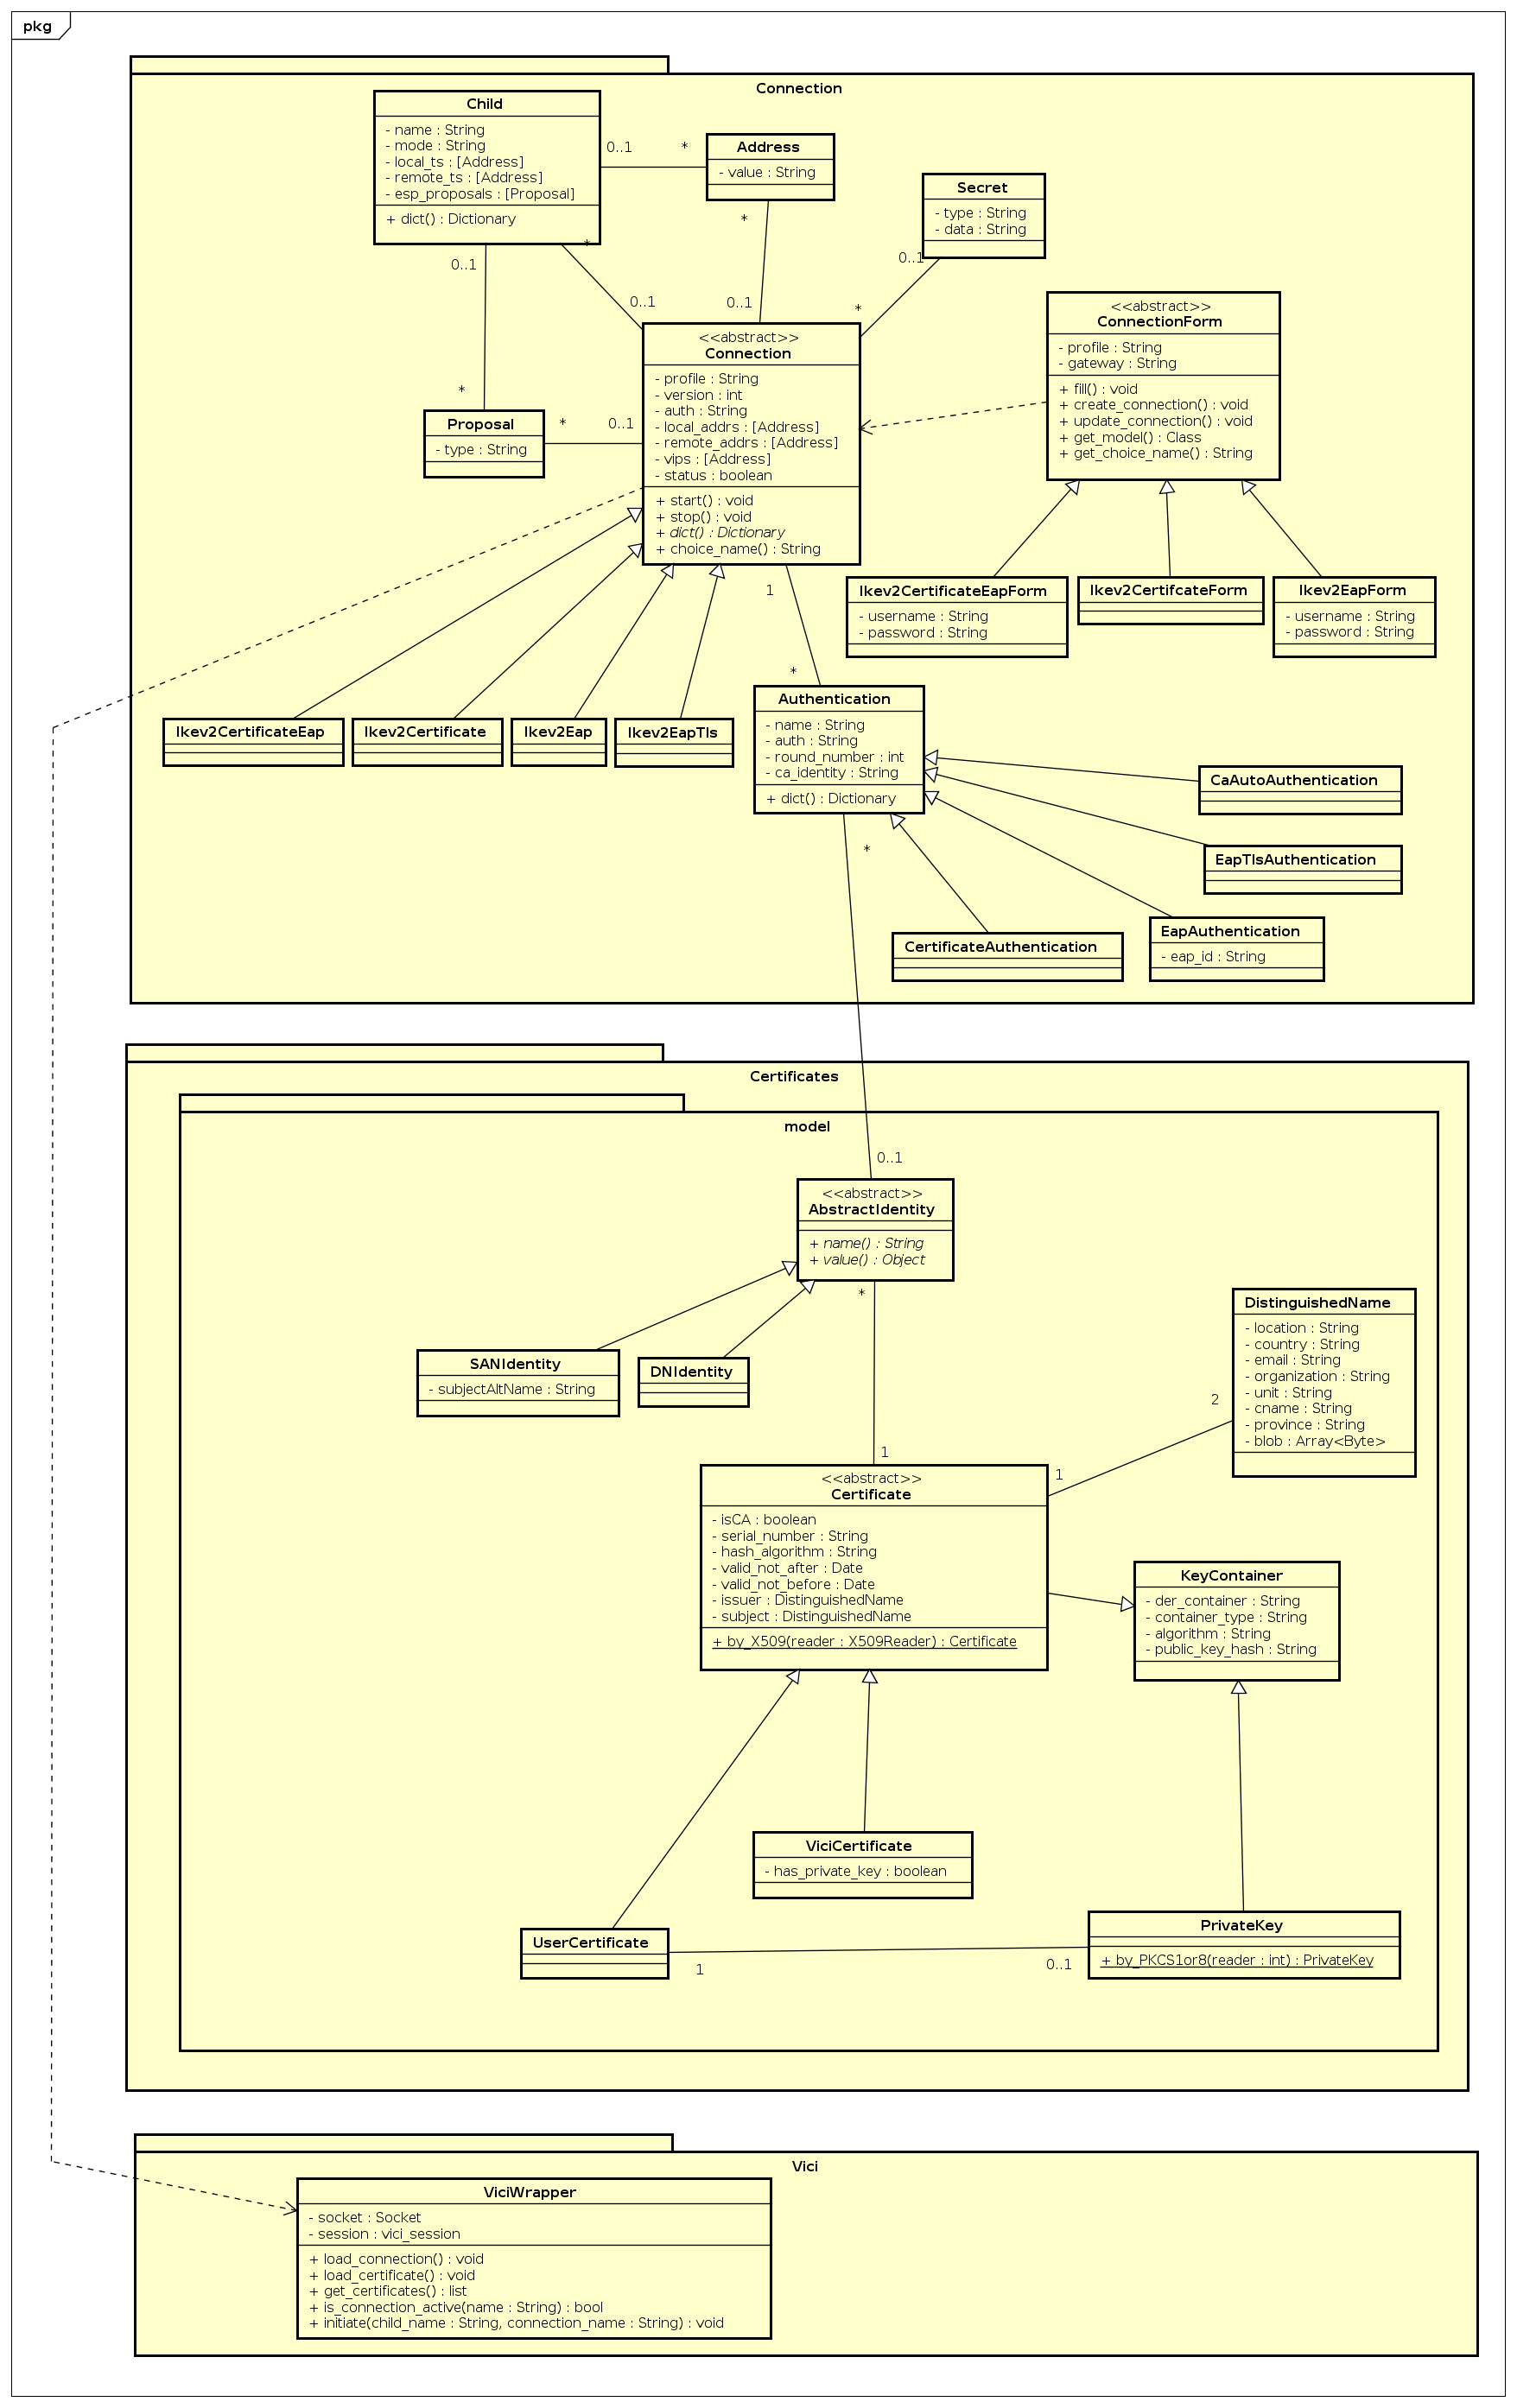
\includegraphics[width=420pt]{images/domain_model_strongman.png}
\caption[Domain Model]{Domain Model}
\end{figure}

Das Domain Model soll im Allgemeinen eine Abstraktion der Vici-Schnittstelle darstellen.
Dabei ist die Connection Klasse zentral. Damit die verschiedenen Authentisierungsmethoden unterstütz werden können, wird von Connection geerbt.

Weiter sind die Certificates ein essentieller Bestandteil, diese sind über die Hilfsklasse AbstractIdentity mit der Authentication verbunden, welche wiederum ein Verbindung zur Connection hat.

\newpage